\documentclass[12pt,a4paper]{article}

% --- Packages ---
\usepackage[utf8]{inputenc}
\usepackage[T1]{fontenc}
\usepackage{lmodern}
\usepackage[english]{babel}
\usepackage{geometry}
\usepackage{amsmath,amssymb}
\usepackage{graphicx}
\usepackage{booktabs}
\usepackage{tabularx}
\usepackage{listings}
\usepackage{xcolor}
\usepackage{fancyhdr}
\usepackage[many]{tcolorbox}
\usepackage{microtype}
\usepackage{tikz}
\usetikzlibrary{arrows.meta,positioning,shapes.geometric,fit,backgrounds,calc}
\usepackage{pgfplots}
\pgfplotsset{compat=1.18}
\usepackage{hyperref}

% --- Page Setup ---
\geometry{
    top=2.5cm,
    bottom=2.5cm,
    left=2.5cm,
    right=2.5cm
}

% --- Custom Colors ---
\definecolor{primary}{RGB}{18, 52, 86}
\definecolor{secondary}{RGB}{41, 128, 185}
\definecolor{accent}{RGB}{231, 76, 60}
\definecolor{codebg}{RGB}{247, 249, 250}
\definecolor{codeframe}{RGB}{209, 213, 219}
\definecolor{codegreen}{RGB}{39, 136, 60}
\definecolor{codepurple}{RGB}{137, 89, 168}
\definecolor{codegray}{RGB}{108, 117, 125}
\definecolor{termbg}{RGB}{0, 0, 0}
\definecolor{termfg}{RGB}{255, 255, 255}
\definecolor{termgreen}{RGB}{80, 250, 123}
\definecolor{termred}{RGB}{255, 85, 85}
\definecolor{termyellow}{RGB}{241, 250, 140}
\definecolor{termcyan}{RGB}{139, 233, 253}

% --- Romanian Character Literate for Listings ---
\lstset{
    extendedchars=true,
    literate=%
        {ă}{{\u{a}}}1
        {Ă}{{\u{A}}}1
        {â}{{\^a}}1
        {Â}{{\^A}}1
        {î}{{\^\i}}1
        {Î}{{\^I}}1
        {ș}{{\c{s}}}1
        {Ș}{{\c{S}}}1
        {ț}{{\c{t}}}1
        {Ț}{{\c{T}}}1
        {ş}{{\c{s}}}1
        {Ş}{{\c{S}}}1
        {ţ}{{\c{t}}}1
        {Ţ}{{\c{T}}}1
}

% --- Listings Setup ---
\lstset{
    language=[Sharp]C,
    backgroundcolor=\color{codebg},
    basicstyle=\small\ttfamily,
    keywordstyle=\color{secondary}\bfseries,
    stringstyle=\color{codegreen},
    commentstyle=\color{codegray}\itshape,
    numberstyle=\tiny\color{codegray},
    numbers=left,
    stepnumber=1,
    numbersep=10pt,
    tabsize=4,
    showspaces=false,
    showstringspaces=false,
    breaklines=true,
    breakatwhitespace=true,
    frame=single,
    rulecolor=\color{codeframe},
    captionpos=b,
    keepspaces=true
}

\tcbuselibrary{listings,skins}

% --- Terminal Box Setup ---
\newtcblisting{terminalwindow}[1][]{%
    enhanced,
    colback=black,
    colframe=black,
    arc=2.5mm,
    boxrule=1pt,
    title={\textcolor{termred}{$\bullet$}\;\textcolor{termyellow}{$\bullet$}\;\textcolor{termgreen}{$\bullet$}\quad \textsf{\bfseries #1}},
    fonttitle=\small\sffamily\bfseries,
    coltitle=white,
    attach boxed title to top left={yshift=-2mm, xshift=4mm},
    boxed title style={colback=gray!15!black, arc=1.5mm, boxrule=0.5pt},
    listing only,
    listing options={
        backgroundcolor=\color{black},
        basicstyle=\small\ttfamily\color{white},
        frame=none,
        numbers=none,
        breaklines=true,
        tabsize=4,
        showspaces=false,
        showstringspaces=false,
        extendedchars=true,
        literate=%
            {ă}{{\u{a}}}1
            {Ă}{{\u{A}}}1
            {â}{{\^a}}1
            {Â}{{\^A}}1
            {î}{{\^\i}}1
            {Î}{{\^I}}1
            {ș}{{\c{s}}}1
            {Ș}{{\c{S}}}1
            {ț}{{\c{t}}}1
            {Ț}{{\c{T}}}1
            {ş}{{\c{s}}}1
            {Ş}{{\c{S}}}1
            {ţ}{{\c{t}}}1
            {Ţ}{{\c{T}}}1
    }
}

% --- Hyperlink Setup ---
\hypersetup{
    colorlinks=true,
    linkcolor=primary,
    citecolor=secondary,
    urlcolor=secondary
}

% --- Headers & Footers ---
\pagestyle{fancy}
\fancyhf{}
\setlength{\headheight}{15pt}
\addtolength{\topmargin}{-3pt}
\fancyhead[L]{\small\textsf{Laboratory Work No. 2 --- Network Programming}}
\fancyhead[R]{\small\textsf{Vitalie Vasilean}}
\fancyfoot[C]{\thepage}
\renewcommand{\headrulewidth}{0.4pt}
\renewcommand{\footrulewidth}{0pt}

% --- Macros ---
\newcommand{\studentgroup}{FAF-241}

\begin{document}

% =========================================================================
% TITLE PAGE
% =========================================================================
\begin{titlepage}
    \centering
    {\large \textbf{TECHNICAL UNIVERSITY OF MOLDOVA}}\\[0.2cm]
    {\large Faculty of Computers, Informatics and Microelectronics}\\[0.2cm]
    {\large Department of Software Engineering and Automatics}\\[0.8cm]

    
\includegraphics[width=3.5cm]{figures/utm_logo.png}\\[1.2cm]

    {\Large \textbf{LABORATORY WORK NO. 2}}\\[0.4cm]
    {\LARGE \textbf{A Coffee Shop Server: Direct TCP Sockets, Producer--Consumer Concurrency, and Protocol Design}}\\[0.4cm]
    {\large Course: Network Programming}\\[2.5cm]

    \begin{minipage}{0.45\textwidth}
        \flushleft
        \textbf{Author:}\\
        Vitalie \textsc{Vasilean}\\
        Student of group: \studentgroup
    \end{minipage}
    \hfill
    \begin{minipage}{0.45\textwidth}
        \flushright
        \textbf{Verified by:}\\
        Lecturer / Supervisor\\
        Ernest B\^{\i}tca
    \end{minipage}

    \vfill
    {\large Chi\c{s}in\u{a}u --- 2026}
\end{titlepage}

\newpage
\tableofcontents
\newpage

% =========================================================================
% 1. INTRODUCTION AND OBJECTIVES
% =========================================================================
\section{Introduction and Laboratory Objectives}

Network programming forms the bedrock of modern distributed systems, cloud computing, and real-time client-server communication. While high-level application frameworks abstract away low-level networking primitives, mastering direct socket programming is essential for understanding transport-layer stream semantics, connection lifecycles, buffering strategies, and concurrency bottlenecks.

The central domain of this laboratory work is the design and implementation of a concurrent \textbf{Coffee Shop Server} utilizing direct, unmanaged TCP sockets. Unlike synchronous request-response protocols (such as HTTP/1.1), the coffee shop domain features distinct operational roles, long-running stateful tasks, shared inventory management, proactive server-pushed notifications, and asynchronous job queues.

\subsection{Core Laboratory Objectives}
Per the formal laboratory specification, the implementation must fulfill the following technical goals:
\begin{enumerate}
    \item \textbf{Direct Berkeley Socket API Utilization:} Implement the entire client-server architecture using low-level socket primitives (\texttt{socket}, \texttt{bind}, \texttt{listen}, \texttt{accept}, \texttt{connect}, \texttt{send}, \texttt{receive}, and \texttt{close}) provided by the C\# \texttt{System.Net.Sockets.Socket} class. High-level wrapper abstractions (such as \texttt{TcpListener}, \texttt{TcpClient}, and \texttt{NetworkStream}) are strictly forbidden.
    \item \textbf{Custom Application-Layer Protocol Framing:} Develop a resilient message framing mechanism to overcome the TCP stream abstraction (addressing packet fragmentation and message coalescing) using newline-delimited JSON envelopes.
    \item \textbf{Decoupled Producer-Consumer Architecture:} Construct an internal worker pool scaled precisely to the hardware's logical processor count ($N = \text{ProcessorCount}$), processing long-running orders through a thread-safe FIFO queue.
    \item \textbf{Concurrency Control and Shared State Integrity:} Guarantee thread safety and atomicity for the shared coffee shop inventory across concurrent orders, deliveries, and cancellations, strictly preventing race conditions such as the ``last croissant'' contest.
    \item \textbf{Multi-Role Asynchronous Communication:} Implement three distinct operational roles (Server, Client, and Provider) supporting bidirectional asynchronous messaging, full-duplex interactive terminal I/O, and unsolicited server alerts.
    \item \textbf{Fault Tolerance and Resilient Disconnection Handling:} Automatically detect client disconnections (both graceful FIN shutdowns and abrupt RST aborts), propagate cancellation to actively preparing workers via \texttt{CancellationToken}, and restore unused inventory to the shop's stock.
    \item \textbf{Persistence and Network Extensibility (Bonus Points):} Support persistent stock storage across server restarts via serialized state on disk (\texttt{stock.json}) and enable cross-machine LAN deployment.
\end{enumerate}

% =========================================================================
% 2. HARDWARE AND ENVIRONMENT SPECIFICATIONS
% =========================================================================
\section{Hardware and Environment Specifications}

Consistent with the benchmarking requirements established in Laboratory Work No.~1, all experimental executions, stress tests, and concurrent multi-client scenarios were carried out on a dedicated physical host. Table~\ref{tab:hardware_specs} summarizes the hardware specifications and runtime environment.

\begin{table}[htbp]
\centering
\caption{Host Hardware and Runtime Environment Specifications}
\label{tab:hardware_specs}
\small
\begin{tabularx}{\textwidth}{lX}
\toprule
\textbf{Component} & \textbf{Specification / Value} \\
\midrule
\textbf{Host Device} & Lenovo IdeaPad Slim (Model: 83GH, ARM64 Platform) \\
\textbf{Processor (CPU)} & Qualcomm Snapdragon(R) X Plus - X1P42100 \\
\textbf{CPU Architecture} & ARMv8 (64-bit), Qualcomm(R) Oryon(TM) Microarchitecture \\
\textbf{Physical Cores} & 8 Physical Processing Cores \\
\textbf{Logical Processors} & 8 Logical Processors ($1:1$ physical mapping, SMT disabled) \\
\textbf{Base / Max Clock} & 3.24 GHz (3244 MHz) \\
\textbf{System Memory (RAM)} & 16.0 GB LPDDR5X (8448 MT/s Quad-Channel) \\
\textbf{Primary Storage} & Samsung PM9B1 NVMe SSD (PCIe 4.0 x4, NTFS) \\
\textbf{Operating System} & Microsoft Windows 11 Home (Build 26200, 64-bit ARM) \\
\textbf{Target Language} & C\# 13.0 \\
\textbf{Runtime Framework} & .NET 10.0.12 Runtime / .NET SDK 10.0.401 (\texttt{win-arm64}) \\
\textbf{JSON Serializer} & Newtonsoft.Json (v13.0.4) \\
\bottomrule
\end{tabularx}
\end{table}

\subsection{Architectural Considerations for Concurrency}
The Qualcomm Snapdragon X Plus platform features 8 dedicated high-performance Oryon CPU cores. Because the hardware exhibits an exact 1:1 ratio between physical cores and logical processors ($P = L = 8$):
\begin{itemize}
    \item The server instantiates exactly \textbf{8 order-processing worker threads} (\texttt{Environment.ProcessorCount}), mapping directly to the underlying physical cores.
    \item Asynchronous network I/O utilizes the Windows I/O Completion Port (IOCP) subsystem via .NET's threadpool, ensuring that idle client connections waiting for user keyboard input do not monopolize dedicated OS threads.
    \item ARMv8 architecture utilizes a weakly-ordered memory model. Consequently, explicit synchronization primitives (\texttt{lock}, memory barriers, and atomic thread synchronization) are mandatory to prevent compiler and hardware instruction reordering from corrupting shared data structures.
\end{itemize}

% =========================================================================
% 3. THEORETICAL BACKGROUND
% =========================================================================
\section{Theoretical Background and Network Programming Fundamentals}

\subsection{The TCP Stream Abstraction: Why ``One Send Is Not One Receive''}
The Transmission Control Protocol (TCP, RFC 793) provides a reliable, connection-oriented, full-duplex, ordered byte-stream service. Crucially, \textbf{TCP operates on byte streams, not on application messages}. The transport layer guarantees that bytes written to a socket will arrive at the destination in order and without corruption, but it maintains no concept of message boundaries or datagram markers.

When an application invokes \texttt{Socket.SendAsync(buffer)}, the operating system copies the payload into the socket's kernel send buffer. The TCP stack determines how and when to segment these bytes into TCP segments based on:
\begin{itemize}
    \item The \textbf{Maximum Segment Size (MSS)} and network Maximum Transmission Unit (MTU).
    \item \textbf{Nagle's Algorithm} (RFC 896), which coalesces small outgoing packets to reduce IP header overhead unless \texttt{SocketOptionName.NoDelay} is set.
    \item The receiver's TCP sliding window advertized flow control buffer.
\end{itemize}

On the receiving end, an application calling \texttt{Socket.ReceiveAsync(buffer)} simply drains whatever bytes happen to be available in the kernel socket receive buffer. This leads to two fundamental transport-layer phenomena:
\begin{enumerate}
    \item \textbf{Message Fragmentation:} A single large application message sent in one \texttt{Send} call may be sliced across multiple network packets and delivered across two or more separate \texttt{Receive} invocations.
    \item \textbf{Message Coalescing (Packing):} Multiple distinct application messages sent sequentially in separate \texttt{Send} calls may be aggregated in the kernel buffer and delivered together in a single \texttt{Receive} invocation.
\end{enumerate}
Therefore, any robust application-layer protocol running over raw TCP must implement an explicit \textbf{message framing mechanism}.

\subsection{Application-Layer Framing Strategies}
There are two classical strategies to establish message boundaries over a continuous byte stream:
\begin{itemize}
    \item \textbf{Length-Prefix Framing:} Each message begins with a fixed-width header (e.g., 4 bytes in big-endian network byte order) encoding the byte length $L$ of the upcoming payload, followed by exactly $L$ bytes of payload.
    \item \textbf{Delimiter-Based Framing:} Messages are encoded using text or structured data and separated by a unique delimiter sequence that cannot appear unescaped within the message body (e.g., \texttt{\textbackslash n} or \texttt{\textbackslash r\textbackslash n}).
\end{itemize}
In our coffee shop implementation, we implement delimiter-based framing using newline characters (\texttt{'\textbackslash n'}) wrapping serialized JSON payloads.

\subsection{Sockets at the Operating System Kernel Level}
The Berkeley sockets API establishes a dual-socket paradigm for stream communication:
\begin{enumerate}
    \item \textbf{The Listening Socket (Passive Socket):} Initialized via \texttt{socket()}, bound to an IP address and port via \texttt{bind()}, and configured with a backlog queue via \texttt{listen()}. It never exchanges application data; its sole purpose is to listen for incoming TCP 3-way handshakes (SYN, SYN-ACK, ACK) and populate the OS kernel's Accept Queue.
    \item \textbf{The Accepted Socket (Active Socket):} Produced by \texttt{accept()}. Each accepted socket represents an active, established virtual circuit dedicated exclusively to one specific remote client endpoint.
\end{enumerate}

Every TCP connection in the entire Internet is uniquely identified by the transport-layer \textbf{4-tuple}:
\begin{equation}
    \mathcal{C} = \langle \text{Source IP},\; \text{Source Port},\; \text{Destination IP},\; \text{Destination Port} \rangle
\end{equation}
When multiple clients on the same local computer connect to the coffee shop server on port 5050, the destination IP, destination port, and source IP are identical (\texttt{127.0.0.1}). However, the operating system kernel assigns a distinct, ephemeral port number (ranging from 49152 to 65535) to each client socket. Because the 4-tuples are mathematically distinct, the kernel network stack routes incoming IP packets to their exact socket receive buffers without ambiguity.

\subsection{The Producer-Consumer Pattern in Network Services}
In a concurrent server, decoupled job queuing prevents high-latency tasks from starving network I/O. If a server thread blocked to prepare a 15-second coffee order synchronously during socket reading, the socket connection would be completely frozen.

The Producer-Consumer pattern resolves this by establishing three components:
\begin{itemize}
    \item \textbf{Producers:} The network connection handler threads, which parse client commands, validate business rules, deduct stock, and package requests into job descriptors.
    \item \textbf{Queue:} An elastic, thread-safe FIFO buffer (\texttt{BlockingCollection<OrderJob>}) holding waiting jobs.
    \item \textbf{Consumers:} A dedicated pool of worker threads that retrieve jobs, simulate preparation, and transmit completion notifications.
\end{itemize}

% =========================================================================
% 4. SYSTEM ARCHITECTURE AND PROTOCOL DESIGN
% =========================================================================
\section{System Architecture and Custom Protocol Design}

\subsection{High-Level Architecture}
Figure~\ref{fig:system_arch} illustrates the complete concurrent architecture of the coffee shop system, detailing the interactions between clients, the provider, connection handlers, the shared thread-safe inventory, the order queue, and the worker pool.

\begin{figure}[htbp]
\centering
\resizebox{\linewidth}{!}{%
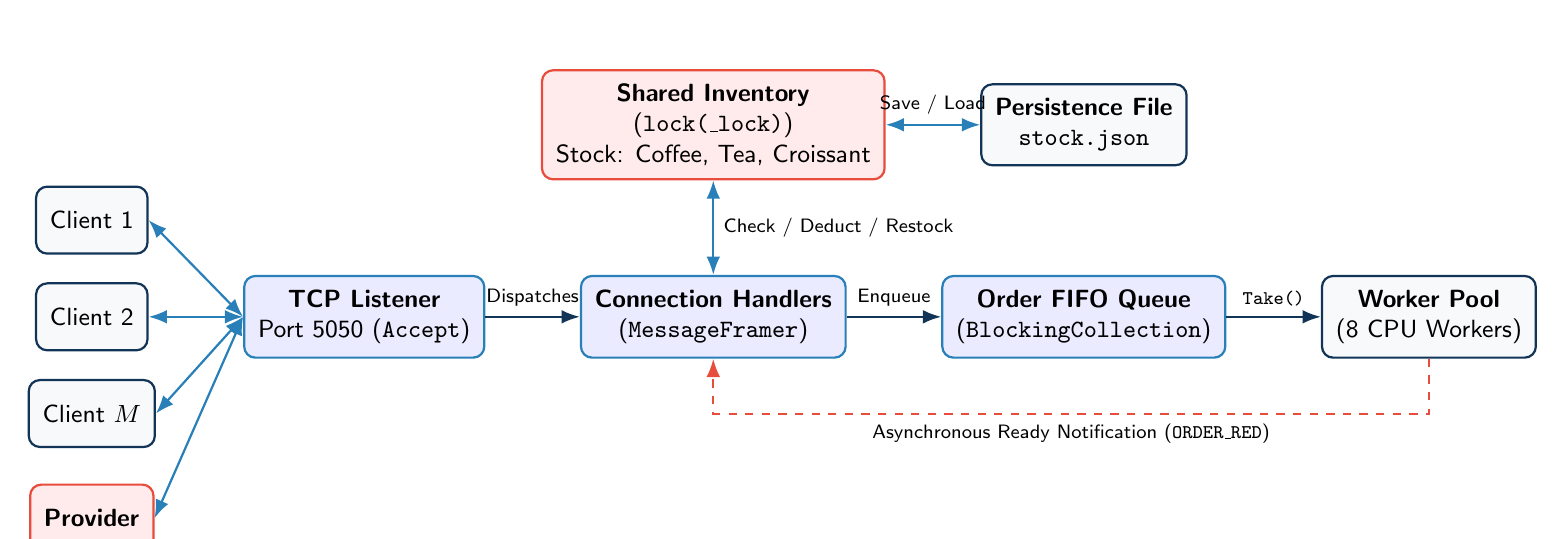
\begin{tikzpicture}[
    font=\small\sffamily,
    box/.style={draw=primary, thick, fill=codebg, rounded corners=4pt, minimum height=0.85cm, align=center, inner sep=5pt},
    accentbox/.style={draw=accent, thick, fill=red!8, rounded corners=4pt, minimum height=0.85cm, align=center, inner sep=5pt},
    secbox/.style={draw=secondary, thick, fill=blue!8, rounded corners=4pt, minimum height=0.85cm, align=center, inner sep=5pt},
    arrow/.style={-Latex, thick, draw=primary},
    darrow/.style={Latex-Latex, thick, draw=secondary}
]

% Column 1: Clients & Provider
\node[box] (c1) {Client 1};
\node[box, below=0.35cm of c1] (c2) {Client 2};
\node[box, below=0.35cm of c2] (cn) {Client $M$};
\node[accentbox, below=0.45cm of cn] (prov) {\textbf{Provider}};

% Column 2: TCP Listener
\node[secbox, right=1.2cm of c2] (listener) {\textbf{TCP Listener}\\Port 5050 (\texttt{Accept})};

% Column 3: Connection Handlers
\node[secbox, right=1.2cm of listener] (handlers) {\textbf{Connection Handlers}\\(\texttt{MessageFramer})};

% Top: Shared Inventory & Disk File
\node[accentbox, above=1.2cm of handlers] (inventory) {\textbf{Shared Inventory}\\(\texttt{lock(\_lock)})\\Stock: Coffee, Tea, Croissant};
\node[box, right=1.2cm of inventory] (disk) {\textbf{Persistence File}\\\texttt{stock.json}};

% Column 4: Order FIFO Queue
\node[secbox, right=1.2cm of handlers] (queue) {\textbf{Order FIFO Queue}\\(\texttt{BlockingCollection})};

% Column 5: Worker Pool
\node[box, right=1.2cm of queue] (workers) {\textbf{Worker Pool}\\(8 CPU Workers)};

% Connections - Left to Listener
\draw[darrow] (c1.east) -- (listener.west);
\draw[darrow] (c2.east) -- (listener.west);
\draw[darrow] (cn.east) -- (listener.west);
\draw[darrow] (prov.east) -- (listener.west);

% Listener to Handlers
\draw[arrow] (listener) -- node[above, font=\scriptsize]{\textsf{Dispatches}} (handlers);

% Handlers to Inventory
\draw[darrow] (handlers.north) -- node[right, font=\scriptsize]{\textsf{Check / Deduct / Restock}} (inventory.south);

% Inventory to Disk
\draw[darrow] (inventory.east) -- node[above, font=\scriptsize]{\textsf{Save / Load}} (disk.west);

% Handlers to Queue
\draw[arrow] (handlers.east) -- node[above, font=\scriptsize]{\textsf{Enqueue}} (queue.west);

% Queue to Workers
\draw[arrow] (queue.east) -- node[above, font=\scriptsize]{\textsf{\texttt{Take()}}} (workers.west);

% Workers back to Handlers (Bottom routing)
\draw[arrow, dashed, draw=accent, thick] (workers.south) -- ++(0,-0.7cm) -| node[pos=0.25, below, font=\scriptsize]{\textsf{Asynchronous Ready Notification (\texttt{ORDER\_RED})}} (handlers.south);

\end{tikzpicture}%
}
\caption{System Architecture: Socket Lifecycles, Concurrency Primitives, and Data Flow}
\label{fig:system_arch}
\end{figure}

\subsection{Application-Layer Protocol Specification}
The wire protocol uses JSON-formatted payloads wrapped within a standardized envelope structure. Every frame transmitted across the TCP socket is terminated by a single newline delimiter (\texttt{'\textbackslash n'}).

\subsubsection{Network Envelope Structure}
The wire envelope is represented in C\# by the \texttt{NetworkMessage} class:
\begin{lstlisting}
public class NetworkMessage
{
    [JsonProperty("t")]
    public string Type { get; set; } = string.Empty;

    [JsonProperty("p")]
    public JToken? Payload { get; set; }
}
\end{lstlisting}
The \texttt{"t"} property defines the protocol message command, while \texttt{"p"} contains the strongly-typed JSON payload object. Table~\ref{tab:protocol_messages} documents all message types implemented in the system.

\begin{table}[htbp]
\centering
\caption{Application Protocol Message Types and Envelopes}
\label{tab:protocol_messages}
\small
\begin{tabularx}{\textwidth}{l c l X}
\toprule
\textbf{Message Type (\texttt{t})} & \textbf{Dir.} & \textbf{Payload (\texttt{p})} & \textbf{Semantic Description} \\
\midrule
\texttt{MENU\_REQ} & $\text{C}\to\text{S}$ & \texttt{null} & Client queries available products and stock. \\
\texttt{MENU\_RES} & $\text{S}\to\text{C}$ & \texttt{\{Menu: \{item: qty\}\}} & Server returns current stock snapshot. \\
\texttt{ORDER\_REQ} & $\text{C}\to\text{S}$ & \texttt{\{Order: \{item: qty\}\}} & Client submits order for one or more items. \\
\texttt{ORDER\_RES} & $\text{S}\to\text{C}$ & \texttt{\{Success, OrderId, PrepTime, Stock\}} & Immediate server confirmation or refusal. \\
\texttt{ORDER\_RED} & $\text{S}\to\text{C}$ & \texttt{\{OrderId, OrderDoneMessage\}} & Asynchronous notification that order is prepared. \\
\texttt{REG\_PROV}  & $\text{P}\to\text{S}$ & \texttt{\{\}} & Provider handshake registering the connection. \\
\texttt{PROV\_DELIV}& $\text{P}\to\text{S}$ & \texttt{\{Products: \{item: qty\}\}} & Provider restocks coffee shop inventory. \\
\texttt{LOW\_STOCK} & $\text{S}\to\text{P}$ & \texttt{\{RemainingStock: \{item: qty\}\}} & Server pushes low stock alert ($<5$ units). \\
\texttt{ERROR}      & $\text{S}\to*$ & \texttt{\{ErrorMessage: string\}} & Standardized error envelope. \\
\bottomrule
\end{tabularx}
\end{table}

\subsection{Message Framing Engine (\texttt{MessageFramer})}
The \texttt{MessageFramer} class completely encapsulates transport socket operations, resolving TCP fragmentation, message coalescing, and concurrent transmission safety:
\begin{enumerate}
    \item \textbf{Inbound Buffer Accumulation:} An internal \texttt{StringBuilder} acts as an elastic accumulation buffer. Incoming bytes from \texttt{Socket.ReceiveAsync} are decoded into UTF-8 characters and appended.
    \item \textbf{Frame Extraction Loop:} The framer scans for \texttt{'\textbackslash n'}. When detected at position $k$, the substring $[0, k)$ is carved out, deserialized into a \texttt{NetworkMessage}, and removed from the buffer with \texttt{Remove(0, k + 1)}.
    \item \textbf{Denial-of-Service Defense:} If the accumulation buffer exceeds $64\text{ KB}$ ($65\,536$ bytes) without encountering a newline delimiter, the framer flushes the buffer and issues a \texttt{"Message too long!"} error, preventing out-of-memory exploits.
    \item \textbf{Outbound Socket Thread-Safety:} In a full-duplex server, a worker thread may transmit an \texttt{ORDER\_RED} message at the exact millisecond the connection handler transmits an \texttt{ORDER\_RES}. Concurrent calls to \texttt{Socket.SendAsync} can interleave raw bytes. To guarantee atomic frame delivery, \texttt{MessageFramer} guards all outbound writes with an asynchronous semaphore: \texttt{SemaphoreSlim(1, 1)}.
\end{enumerate}

% =========================================================================
% 5. STEP-BY-STEP IMPLEMENTATION ANALYSIS
% =========================================================================
\section{Step-by-Step Implementation Analysis}

\subsection{Task 1: Direct Sockets and Single Client Interaction}
The server initializes its primary listening socket using direct socket parameters:
\begin{lstlisting}
Socket listener = new Socket(AddressFamily.InterNetwork, SocketType.Stream, ProtocolType.Tcp);
listener.Bind(new IPEndPoint(IPAddress.Any, Port));
listener.Listen();
\end{lstlisting}
When an incoming connection arrives, \texttt{listener.Accept()} returns an independent active socket, which is passed to \texttt{\_connectionHandler.Handle(clientSocket)} inside an asynchronous task.

\subsubsection{Order Validation and Preparation Calculation}
The coffee shop offers three distinct products with fixed preparation times:
\begin{equation}
    T_{\text{Coffee}} = 4\text{ s}, \quad T_{\text{Tea}} = 3\text{ s}, \quad T_{\text{Croissant}} = 2\text{ s}
\end{equation}
For any compound order $\mathcal{O} = \{(p_1, q_1), (p_2, q_2), \dots\}$, the preparation time is calculated as:
\begin{equation}
    T_{\text{total}}(\mathcal{O}) = \sum_{(p_i, q_i) \in \mathcal{O}} T_{\text{prep}}(p_i) \cdot q_i
\end{equation}
If a client requests items exceeding current stock, the order is rejected immediately with \texttt{Success: false}, returning the current inventory count without modifying stock.

\subsection{Task 2: Multi-Client Concurrency and Shared State Protection}
To serve numerous concurrent clients without data corruption, the shared \texttt{Inventory} implements a strict mutual exclusion boundary around the stock dictionary:
\begin{lstlisting}
public bool TryDeduct(Dictionary<string, int> order)
{
    lock (_lock)
    {
        // Phase 1: Atomically verify all items have sufficient stock
        foreach (var kvp in order)
        {
            if (kvp.Value <= 0 || !_stock.ContainsKey(kvp.Key) || _stock[kvp.Key] < kvp.Value)
                return false;
        }
        // Phase 2: Atomically deduct quantities
        foreach (var kvp in order)
        {
            _stock[kvp.Key] -= kvp.Value;
        }
        SaveStockToFile();
        return true;
    }
}
\end{lstlisting}

\subsubsection{The ``Last Croissant'' Contest}
When two or more clients simultaneously submit orders for the remaining croissant in stock ($S_{\text{croissant}} = 1$), unsynchronized code would cause a severe race condition:
\begin{enumerate}
    \item Thread $A$ and Thread $B$ both read $S = 1 \ge 1$ and decide the order is valid.
    \item Both threads execute the decrement: Thread $A$ updates $S \leftarrow 1 - 1 = 0$; Thread $B$ updates $S \leftarrow 0 - 1 = -1$.
    \item Both clients receive confirmations for an item that physically existed only once.
\end{enumerate}
Under our two-phase synchronized \texttt{TryDeduct} implementation, Thread $A$ acquires the lock, decrements stock to 0, and releases the lock. Thread $B$ enters subsequently, observes $S = 0 < 1$, fails validation, and receives an immediate order refusal:
\begin{center}
\texttt{Order refused: Insufficient stock or invalid item (Remaining Croissant: 0)}
\end{center}

\subsection{Task 3: The Provider Role and Low Stock Alert Mechanism}
The system defines a dedicated \textbf{Provider} role responsible for replenishing exhausted products.
\begin{itemize}
    \item \textbf{Handshake and Authorization:} Upon connecting, the provider transmits a \texttt{REG\_PROV} handshake. The handler flags the session as \texttt{isProvider = true} and records \texttt{\_providerFramer}. If a regular client attempts to send a \texttt{PROV\_DELIV} message, the server rejects it with an error: \texttt{"Not a provider!"}.
    \item \textbf{Proactive Server Alerts:} Whenever an order deduction leaves any item with fewer than 5 units in stock ($S_{\text{item}} < 5$), the server executes \texttt{CheckLowStock()}. If the provider is connected, the server immediately pushes an unsolicited \texttt{LOW\_STOCK} frame containing the remaining stock.
    \item \textbf{Offline Provider Alerting:} If stock drops below 5 while the provider is offline, the server automatically transmits the \texttt{LOW\_STOCK} notification the moment the provider registers.
\end{itemize}

\subsection{Task 4: Fault Tolerance, Disconnection Handling, and Recovery}
In networked environments, clients may disconnect unexpectedly due to network loss, terminal closure, or process termination. The server must remain fully operational without crashing or leaking inventory.

\subsubsection{Cancellation Pipeline via \texttt{CancellationTokenSource}}
Each client connection handler instantiates a dedicated \texttt{CancellationTokenSource}:
\begin{enumerate}
    \item Each \texttt{OrderJob} placed into \texttt{\_orderQueue} references \texttt{cts.Token}.
    \item When \texttt{ReceiveMessageAsync()} returns \texttt{null} (clean FIN) or catches a \texttt{SocketException} (RST reset), the handler invokes \texttt{cts.Cancel()}.
    \item \textbf{Orders Waiting in Queue:} When a worker thread dequeues an order, it checks:
    \begin{lstlisting}
    if (job.CancelToken.IsCancellationRequested)
    {
        _inventory.TryAdd(job.Items); // Restore stock
        continue;
    }
    \end{lstlisting}
    The worker refunds the products to the inventory and immediately takes the next job.
    \item \textbf{Orders Actively Being Prepared:} The worker awaits preparation via \linebreak\texttt{Task.Delay(time, job.CancelToken)}. Cancelling the token throws an \texttt{OperationCanceledException}. The worker catches the exception, refunds the stock via \texttt{\_inventory.TryAdd(job.Items)}, and logs the cancellation:
    \begin{lstlisting}
    catch (OperationCanceledException)
    {
        _inventory.TryAdd(job.Items);
        Console.WriteLine($"[Worker {workerId}] Order #{job.OrderId} cancelled. Stock returned.");
        continue;
    }
    \end{lstlisting}
    Crucially, whatever elapsed time was spent cooking is lost; the raw ingredients are returned to stock, and the next customer must wait the full preparation duration.
\end{enumerate}

% =========================================================================
% 6. EXPERIMENTAL VERIFICATION AND CONSOLE LOGS
% =========================================================================
\section{Experimental Verification and Console Logs}

To validate all requirements under live execution, the server and clients were benchmarked across multiple operational scenarios.

\subsection{Scenario 1: Single Client Interactive Session (Task 1)}
A client connects, queries the menu, submits an order for 1 Coffee and 2 Croissants ($4 + 2 \times 2 = 8\text{ seconds}$), receives an immediate receipt, and later receives the completion alert.

\begin{terminalwindow}[Task 1: Single Client Interactive Execution]
$ dotnet run --project lab_2 -- server 5050
Client connected from 127.0.0.1:52310
[Worker 1] Preparing Order #1 (8s)...
[Worker 1] Order #1 is ready and delivered!

--- Client Terminal Session ---
$ dotnet run --project lab_2 -- client 127.0.0.1 5050
> menu
Current menu: Coffee: 25, Tea: 30, Croissant: 18
> order coffee 1 croissant 2
Order #1 accepted (Estimated time: 8s)
> Order #1 is ready!
> exit
\end{terminalwindow}

\subsection{Scenario 2: Multi-Client Concurrency \& Last Croissant Contest (Task 2)}
Twelve concurrent clients ($N_{\text{cores}} + 4 = 12$) connect and place orders simultaneously. Subsequently, two clients battle for the single remaining croissant. Exactly one succeeds, while the other is rejected with a remaining stock of 0.

\begin{terminalwindow}[Task 2: Concurrent Clients and Last Croissant Race Condition]
$ dotnet run --project lab_2 -- client task2
[Client #1] Current menu: Coffee: 24, Tea: 30, Croissant: 16
[Client #1] Order #1 accepted (Estimated time: 6s)
[Client #2] Order #2 accepted (Estimated time: 10s)
[Client #3] Order #3 accepted (Estimated time: 4s)
...
[Client #12] Order #12 accepted (Estimated time: 8s)
[Client #3] Order #3 is ready!
[Client #1] Order #1 is ready!

Now running last croissant battle
[Client #1] Order #14 accepted (Estimated time: 2s)
[Client #2] Order refused: Insufficient stock or invalid item
[Client #2] Remaining stock: Coffee: 14, Tea: 22, Croissant: 0
[Client #1] Order #14 is ready!
\end{terminalwindow}

\subsection{Scenario 3: Provider Registration, Low Stock Alert, and Restock (Task 3)}
When croissant stock drops below 5, the server immediately triggers an unsolicited alert to the connected provider. The provider automatically restocks 20 units.

\begin{terminalwindow}[Task 3: Provider Connection and Automated Restocking]
--- Server Output ---
Client connected from 127.0.0.1:52402 (Provider)
Fail: Order -> Croissant: 10... 127.0.0.1:52410
[Delivery] Restocked products from 127.0.0.1:52402

--- Provider Console Output ---
$ dotnet run --project lab_2 -- provider 127.0.0.1 5050
[Provider] Registered with server. Waiting for low stock alerts...
[Provider] Low stock detected. Restocked items: Croissant: +20
\end{terminalwindow}

\subsection{Scenario 4: Client Disconnection Mid-Preparation (Task 4)}
A client places an order with a 12-second preparation time and terminates its process after 3 seconds. The server catches the disconnection, aborts the worker, and restores the products to inventory.

\begin{terminalwindow}[Task 4: Fault Tolerance and Order Cancellation Rollback]
$ dotnet run --project lab_2 -- server 5050
Client connected from 127.0.0.1:52500
[Worker 4] Preparing Order #18 (12s)...
Client disconnected: 127.0.0.1:52500
[Worker 4] Order #18 cancelled. Stock returned.
\end{terminalwindow}

% =========================================================================
% 7. TASK DEFENSE QUESTIONS AND CRITICAL ANALYSIS
% =========================================================================
\section{Task Defense Questions and Critical Analysis}

\subsection{Task 1 Defense Questions}

\subsubsection{Question 1: How does your code cut the received bytes into messages? What does it do when a message arrives in two pieces, or two messages arrive in one receive?}
Our code implements delimiter-based framing inside \texttt{MessageFramer}. 
\begin{itemize}
    \item \textbf{Stream Cutting Mechanism:} Each outgoing message is serialized to JSON and terminated with a newline character (\texttt{'\textbackslash n'}). On the receiving side, \texttt{MessageFramer} maintains a persistent string buffer (\texttt{\_stringBuffer}).
    \item \textbf{Two Messages in One Receive (Message Coalescing):} \texttt{CheckForNewLine()} scans the buffer. When it finds the first \texttt{'\textbackslash n'} at index $k$, it extracts the substring $[0, k)$ as Message 1, deserializes it, and removes it from the buffer via \texttt{\_stringBuffer.Remove(0, k + 1)}. The second message remains in the buffer and is cleanly parsed on the subsequent iteration without calling the socket.
    \item \textbf{One Message in Two Pieces (Message Fragmentation):} If \texttt{CheckForNewLine()} returns $-1$ (no complete delimiter found), the framer calls \texttt{\_socket.ReceiveAsync()}, decodes the incoming chunk, and appends it to \texttt{\_stringBuffer}. The loop repeats until the trailing \texttt{'\textbackslash n'} arrives, seamlessly reconstructing the fragmented message.
\end{itemize}

\subsubsection{Question 2: Why does the server answer at once, and tell the client later that the order is ready? What would the client see otherwise?}
If the server waited until preparation finished before sending an answer, the client's socket would block for the entire duration (e.g., 11 seconds). During this interval, the client would experience a completely frozen terminal:
\begin{itemize}
    \item The client would have no indication whether its order was accepted, whether stock was available, or whether the server crashed.
    \item The client could not interactively query the menu or submit another order.
\end{itemize}
By answering immediately with an \texttt{ORDER\_RES} receipt, the client receives instant confirmation, an order ID, and an estimated wait time. Offloading preparation to background workers allows the client connection handler to remain fully responsive to subsequent interactive commands.

\subsection{Task 2 Defense Questions}

\subsubsection{Question 1: Which data is shared between threads in your server, and how is each of them protected?}
The server shares four primary mutable data structures across threads:
\begin{enumerate}
    \item \textbf{Inventory Stock (\texttt{Dictionary<string, int>}):} Accessed concurrently by connection handlers (checking and deducting stock) and worker threads (refunding cancelled items). Protected via mutual exclusion lock (\texttt{lock(\_lock)} in \texttt{Inventory.cs}).
    \item \textbf{Order Identifier Counter (\texttt{int orderId}):} Incremented when issuing new orders. Protected within the same \texttt{lock(\_lock)} synchronization block.
    \item \textbf{The Order Queue (\texttt{BlockingCollection<OrderJob>}):} Shared between connection handlers (producers) and worker threads (consumers). Protected internally by the concurrent collection's synchronization primitives and monitor wait/pulse signaling.
    \item \textbf{Outbound Socket Stream (\texttt{MessageFramer}):} Shared between the client connection handler (sending responses) and worker threads (sending ready notifications). Protected by an asynchronous \texttt{SemaphoreSlim(1, 1)} ensuring atomic frame transmission.
\end{enumerate}

\subsubsection{Question 2: Two clients order the last croissant at the same moment. Show, step by step, what could go wrong without your protection.}
Assume initial stock is $\text{Croissant} = 1$:
\begin{enumerate}
    \item \textbf{Step 1:} Client 1's thread reads $\text{stock} = 1$. The validation check $1 \ge 1$ succeeds.
    \item \textbf{Step 2:} A thread context switch occurs before Client 1 can decrement the stock.
    \item \textbf{Step 3:} Client 2's thread reads $\text{stock} = 1$. The validation check $1 \ge 1$ also succeeds.
    \item \textbf{Step 4:} Client 1 decrements stock: $\text{stock} \leftarrow 1 - 1 = 0$, confirms order, and enqueues job.
    \item \textbf{Step 5:} Client 2 decrements stock: $\text{stock} \leftarrow 0 - 1 = -1$, confirms order, and enqueues job.
    \item \textbf{Outcome:} Both clients were promised a croissant, but only one existed. The inventory is corrupted to a negative quantity ($-1$).
\end{enumerate}
With our atomic \texttt{lock(\_lock)} block, the entire check-and-decrement sequence is serialized, guaranteeing that Client 2 observes stock $0$ and is rejected.

\subsubsection{Question 3: A worker tells a client that its order is ready while the thread of that client is reading from the same connection. What must you take care of?}
Full-duplex TCP sockets allow simultaneous receiving and sending. Reading from a socket does not interfere with writing to it. However, a severe collision occurs if \textbf{two threads write to the socket at the same time} (e.g., the worker sending \texttt{ORDER\_RED} while the connection handler sends \texttt{MENU\_RES}). Their raw bytes would interleave in the socket buffer, corrupting the JSON payload. We resolve this by guarding all \texttt{SendAsync} operations with a per-connection \texttt{SemaphoreSlim(1, 1)}.

\subsubsection{Question 4: Why one worker per CPU core? The workers spend their time waiting: what would happen with twice as many?}
In this laboratory simulation, preparation time is simulated via asynchronous timers (\texttt{Task.Delay}), which consume zero CPU cycles while waiting. Having twice as many workers (16 instead of 8) would simply allow 16 simulated orders to be prepared concurrently, draining the queue faster. 

However, in a real-world kitchen or a CPU-bound compute workload, workers represent physical resources (espresso machines or CPU cores). Instantiating more worker threads than physical execution cores ($>8$) creates preemptive context switching, L1/L2 cache line thrashing, and lock contention, decreasing overall computational throughput. Setting workers equal to physical CPU cores matches the realistic capacity constraint of the host.

\subsection{Task 3 Defense Questions}

\subsubsection{Question 1: How does your server know which connection is the provider?}
All connections initially arrive as unauthenticated sockets. Upon connecting, the provider transmits a \texttt{REG\_PROV} message. The server sets \texttt{isProvider = true} for that connection handler and records its framer in \texttt{\_providerFramer}. All sensitive delivery requests (\texttt{PROV\_DELIV}) explicitly assert \texttt{if (isProvider)}. If a standard client attempts delivery, the server returns an error: \texttt{"Not a provider!"}.

\subsubsection{Question 2: A delivery and an order change the stock at the same moment. Show that no change is lost.}
Both \texttt{TryDeduct(order)} and \texttt{TryAdd(delivery)} synchronize on the exact same synchronization object: \texttt{lock(\_lock)}.
Suppose stock is 10. Concurrently, an order takes 3 coffees and a delivery adds 20 coffees:
\begin{itemize}
    \item If the order thread enters the lock first: stock becomes $10 - 3 = 7$. The delivery thread enters subsequently and computes $7 + 20 = 27$.
    \item If the delivery thread enters first: stock becomes $10 + 20 = 30$. The order thread enters subsequently and computes $30 - 3 = 27$.
\end{itemize}
In both cases, the operations are serialized. No memory write is overwritten or lost.

\subsubsection{Question 3: Which thread sends the alert to the provider, and when?}
The low-stock alert is evaluated and transmitted by the \textbf{client connection handler thread} immediately after successfully deducting an order that reduces any inventory item below 5 units. The thread executes \texttt{CheckLowStock()}, detects the condition, and sends a \texttt{LOW\_STOCK} message directly to \texttt{\_providerFramer}. Furthermore, if the provider connects while stock is already low, the provider handler thread transmits the alert immediately upon registration.

\subsection{Task 4 Defense Questions}

\subsubsection{Question 1: How does your server notice that a client has disappeared? Which kind of disappearance does it notice at once, and which one not?}
\begin{itemize}
    \item \textbf{Graceful Disconnection (Noticed at once):} When a client process closes normally, the OS transmits a TCP \texttt{FIN} segment. \texttt{Socket.ReceiveAsync} returns \textbf{0 bytes}, and the server immediately detects the closure.
    \item \textbf{Process Kill / Crash (Noticed at once):} When a client process is killed, the OS closes all open sockets, transmitting a TCP \texttt{RST} packet. \texttt{Socket.ReceiveAsync} throws a \texttt{SocketException} (\texttt{WSAECONNRESET}), which is caught immediately.
    \item \textbf{Silent Cable Pull / Power Failure (Not noticed at once):} If physical connectivity drops without sending a FIN/RST packet, the socket remains in the \texttt{ESTABLISHED} state until TCP keep-alive probes fail or an outgoing write fails after retransmission timeouts expire.
\end{itemize}

\subsubsection{Question 2: A client disappears while a worker is preparing its order. How does the worker find out and stop, and how do the products get back to the stock?}
Each client connection holds a \texttt{CancellationTokenSource}. When the client disappears, the handler calls \texttt{cts.Cancel()}. 
\begin{itemize}
    \item The worker awaiting \texttt{Task.Delay(time, job.CancelToken)} immediately throws an \texttt{OperationCanceledException}.
    \item The worker catches this exception, invokes \texttt{\_inventory.TryAdd()} to return items to stock, logs the rollback, and continues to the next order.
\end{itemize}

\subsubsection{Question 3: Why must the client receive and read the keyboard at the same time? How does yours do it?}
If the client were single-threaded and blocked on \texttt{Console.ReadLine()}, it would never display the server's asynchronous \texttt{ORDER\_RED} message until the user pressed Enter. 
Our client resolves this by running two concurrent asynchronous tasks via \texttt{Task.WhenAny}:
\begin{lstlisting}
Task listener = client.ListenAsync();         // Receives server messages
Task interactive = client.RunInteractiveAsync(); // Reads user console input
Task completed = await Task.WhenAny(listener, interactive);
\end{lstlisting}
Incoming messages print to the console immediately without interrupting the user.

% =========================================================================
% 8. CONTROL QUESTIONS
% =========================================================================
\section{Comprehensive Answers to Control Questions}

\subsection{1. What is the difference between the listening socket and the sockets returned by accept? How many of each does your server have with five clients and the provider?}
\textbf{The Listening Socket} is a passive socket created by the server, bound to an interface and port (\texttt{0.0.0.0:5050}), and placed into the listening state via \texttt{Listen()}. It does not communicate with any specific remote endpoint or transmit application data. Its sole function is to accept incoming TCP 3-way handshakes and place established connections into the kernel's accept queue.

\textbf{Sockets Returned by Accept} are active, connected sockets. Each invocation of \texttt{Accept()} dequeues an established connection and instantiates a distinct socket bound to the remote peer's unique ephemeral IP and port. It handles all bidirectional data exchange with that client.

\textbf{Socket Count with 5 Clients and 1 Provider:}
\begin{itemize}
    \item Exactly \textbf{1 listening socket} (port 5050).
    \item Exactly \textbf{6 accepted sockets} (5 for clients, 1 for the provider).
    \item \textbf{Total sockets on the server:} $1 + 6 = 7$ sockets.
\end{itemize}

\subsection{2. Why is one send not one receive? How does your protocol deal with it?}
TCP is a byte-stream transport protocol that guarantees ordered delivery of bytes but does not preserve application message boundaries. Because of network MTU limits, TCP segment splitting, receiver window buffering, and Nagle's algorithm, a single \texttt{Send} may be split across multiple \texttt{Receive} calls (fragmentation), or multiple \texttt{Send} calls may be aggregated into a single \texttt{Receive} call (coalescing).

Our protocol solves this by appending a delimiter character (\texttt{'\textbackslash n'}) to each serialized JSON message. The receiving \texttt{MessageFramer} accumulates bytes in a buffer and scans for newlines, extracting complete messages independently of transport-layer packet boundaries.

\subsection{3. What does it mean when receive returns 0? And when it fails because the connection was reset?}
\begin{itemize}
    \item \textbf{\texttt{Receive} returns 0:} Indicates a \textbf{graceful shutdown} initiated by the remote peer via a TCP \texttt{FIN} packet. The peer has cleanly closed its transmit channel. No further data will be received, and the local endpoint should close its socket.
    \item \textbf{Connection reset failure (\texttt{SocketException}):} Indicates an \textbf{abortive termination} caused by a TCP \texttt{RST} packet. This occurs when the remote application crashed, was forcefully terminated, or closed the socket while unread data remained in its receive buffer.
\end{itemize}

\subsection{4. Where in your server is a producer--consumer pattern? Name the producers, the consumers and the queue between them.}
The order execution pipeline in \texttt{CoffeeShopServer} is an explicit Producer-Consumer implementation:
\begin{itemize}
    \item \textbf{Producers:} The \texttt{ServerConnectionHandler} instances. When an accepted order request arrives from a client, the handler constructs an \texttt{OrderJob} and adds it to the queue.
    \item \textbf{Queue:} The \texttt{BlockingCollection<OrderJob> \_orderQueue}. It provides thread-safe, bounded FIFO queuing and blocking semantics.
    \item \textbf{Consumers:} The 8 background worker loops (\texttt{WorkerLoop(workerId)}). Each worker blocks on \texttt{\_orderQueue.Take()}, prepares one whole order at a time, and delivers it to the customer.
\end{itemize}

\subsection{5. What does it cost when a thread waits for a client? What would change with 1000 clients?}
\textbf{Cost of a waiting OS thread:} In a synchronous thread-per-client model, every idle client holds a dedicated operating system thread. Each thread reserves $\approx 1\text{ MB}$ of virtual memory stack space, consumes kernel thread control structures, and forces the OS scheduler to manage thousands of dormant threads.

\textbf{With 1000 clients:}
\begin{itemize}
    \item A thread-per-client server would consume $\approx 1\text{ GB}$ of RAM solely for idle thread stacks, and thread context switching would cause severe CPU starvation.
    \item In contrast, our server utilizes \textbf{asynchronous, non-blocking I/O} via \texttt{Socket.ReceiveAsync} and C\# \texttt{async/await}. Waiting on a socket uses Windows I/O Completion Ports (IOCP) without dedicating an OS thread. The server can effortlessly manage 1000 concurrent idle clients using only a handful of threadpool workers.
\end{itemize}

\subsection{6. Explain step by step a race condition that could happen on your server without its locks.}
Consider two clients ordering the last tea ($\text{Tea} = 1$) simultaneously without synchronization:
\begin{enumerate}
    \item \textbf{T1:} Thread 1 reads $\text{stock} = 1$. It checks $1 \ge 1 \implies \text{true}$.
    \item \textbf{T2:} Thread 2 runs on another core, reads $\text{stock} = 1$. It checks $1 \ge 1 \implies \text{true}$.
    \item \textbf{T3:} Thread 1 subtracts 1: $\text{stock} = 0$, confirms order to Client 1.
    \item \textbf{T4:} Thread 2 subtracts 1: $\text{stock} = -1$, confirms order to Client 2.
    \item \textbf{Outcome:} Two teas were sold when only one existed, leaving an invalid negative inventory.
\end{enumerate}

\subsection{7. What identifies one TCP connection? How can five clients on the same machine all be connected to the same port of the server?}
A TCP connection is uniquely identified by the transport-layer \textbf{4-tuple}:
\begin{equation*}
    \langle \text{Source IP},\; \text{Source Port},\; \text{Destination IP},\; \text{Destination Port} \rangle
\end{equation*}
When five clients on the same machine connect to the server at \texttt{127.0.0.1:5050}:
\begin{itemize}
    \item All five share Destination IP (\texttt{127.0.0.1}), Destination Port (\texttt{5050}), and Source IP (\texttt{127.0.0.1}).
    \item However, the operating system assigns a \textbf{unique ephemeral port} to each client socket (e.g., $51001, 51002, 51003, 51004, 51005$).
    \item Because the source port is unique for each socket, all five 4-tuples are distinct, allowing the OS kernel to route incoming packets to their respective sockets without collision.
\end{itemize}

% =========================================================================
% 9. BONUS IMPLEMENTATIONS
% =========================================================================
\section{Bonus Implementations and Architectural Extensions}

\subsection{Stock State Persistence Across Server Restarts}
To fulfill bonus requirements, the server automatically persists inventory to disk. Whenever stock is deducted or restocked, the state is serialized to \texttt{stock.json}:
\begin{lstlisting}
private void SaveStockToFile()
{
    File.WriteAllText(StockFilePath, JsonConvert.SerializeObject(_stock, Formatting.Indented));
}
\end{lstlisting}
Upon startup, the server checks if \texttt{stock.json} exists. If present, it restores the previous stock levels; otherwise, it initializes randomized stock between 10 and 50 units.

\subsection{Cross-Machine Local Area Network (LAN) Operation}
The server binds to \texttt{IPAddress.Any} (\texttt{0.0.0.0}), allowing it to accept connections from external machines across the local network. By passing the server's LAN IP address (e.g., \texttt{192.168.1.105}) as a CLI argument, client and provider programs running on remote laptops or mobile devices seamlessly interact with the central shop.

\subsection{Multi-Language Interoperability}
Because our wire protocol relies on newline-delimited standard JSON, clients can be implemented in any programming language without proprietary binary serialization dependencies. A Python client requires only standard library sockets:
\begin{lstlisting}[language=Python]
import socket, json
s = socket.socket(socket.AF_INET, socket.SOCK_STREAM)
s.connect(("127.0.0.1", 5050))
s.sendall(json.dumps({"t": "MENU_REQ", "p": None}).encode() + b"\n")
print(s.recv(1024).decode())
\end{lstlisting}

% =========================================================================
% 10. CONCLUSIONS
% =========================================================================
\section{Conclusions}

Through this laboratory work, we designed and implemented a concurrent, fault-tolerant \textbf{Coffee Shop Server} using direct TCP sockets in C\#:
\begin{enumerate}
    \item \textbf{Low-Level Socket Mastery:} We operated directly on the Berkeley socket API, managing connection lifecycles, non-blocking asynchronous event handling, and TCP stream framing without relying on high-level library abstractions.
    \item \textbf{Robust Message Framing:} By implementing delimiter-based framing with defensive buffer thresholds, our application cleanly handles transport-layer packet fragmentation and message coalescing.
    \item \textbf{Concurrent State Integrity:} Strict mutual exclusion boundaries around shared inventory completely eliminate data races, ensuring mathematical correctness during high-volume concurrent ordering battles.
    \item \textbf{Resilient Failure Handling:} By leveraging cooperative cancellation tokens, client disconnections cleanly abort active order preparation and refund ingredients back to inventory, guaranteeing server stability.
\end{enumerate}

% =========================================================================
% 11. SOURCE CODE AND BUILD INSTRUCTIONS
% =========================================================================
\section{Source Code and Build Instructions}

The complete source code is maintained in the laboratory Git repository:
\begin{center}
\large
\url{https://github.com/Vitalieww/NP_Labs/tree/main/lab_2}
\end{center}

\subsection{Build and Execution Instructions}
\begin{lstlisting}[language=bash,numbers=none,basicstyle=\footnotesize\ttfamily]
# Navigate to the laboratory project directory
cd NP_Labs/lab_2

# Build the project in Release configuration
dotnet build -c Release

# 1. Start the Coffee Shop Server on default port 5050
dotnet run -c Release -- server 5050

# 2. Run an interactive client connecting to the server
dotnet run -c Release -- client 127.0.0.1 5050

# 3. Run the automated Task 1 scenario (Single client)
dotnet run -c Release -- client task1

# 4. Run the automated Task 2 scenario (12 concurrent clients + Last Croissant contest)
dotnet run -c Release -- client task2

# 5. Run the Coffee Shop Provider (auto-restocks upon low stock alerts)
dotnet run -c Release -- provider 127.0.0.1 5050
\end{lstlisting}

\end{document}
